\section{Kinematik}
\subsection{Geradlinige Bewegungen(Translation)}

\begin{shaded}
\begin{align*}
	a(t)&=a_0=\frac{\diff v}{\diff t}=\dot{v}=\ddot{s} \\
	v(t)&=a_0\cdot t+v_0=\frac{\diff s}{\diff t}=\dot{s} \\
	s(t)&=\frac{1}{2}a_0\cdot t^2+v_0\cdot t+s_0
\end{align*}
\end{shaded}

\subsection{Kreisbewegungen(Rotation)}

\begin{boxleft}
\bla{Winkelgrößen}
\des[\radian\per\second\tothe{2}]{\alpha}{Winkelbeschleunigung}\\
\des[\radian\per\second\tothe{1}]{\omega}{Winkelgeschwindigkeit}\\
\des[\radian]{\varphi}{Drehwinkel}
\end{boxleft}\begin{boxrightshaded}
\begin{align*}
\alpha(t)&=\alpha_0=\frac{\diff \omega}{\diff t}=\dot{\omega}=\ddot{\varphi} \\
\omega(t)&=\alpha_0\cdot t+\omega_0=\frac{\diff \varphi}{\diff t}=\dot{\varphi} \\
\varphi(t)&=\frac{1}{2}\alpha_0\cdot t^2+\omega_0\cdot t+\varphi_0
\end{align*}
\end{boxrightshaded}

\begin{boxleft}
\bla{Bahngrößen}
\des[\meter\per\second\tothe{2}]{a_t}{Beschleunigung(tan)}\\
\des[\meter\per\second\tothe{1}]{v}{Geschwindugkeit}\\
\des[\meter]{s}{Weg}
\end{boxleft}\begin{boxrightshaded}
\begin{align*}
a_t(t)&=a_0=\frac{\diff v}{\diff t}=\dot{v}=\ddot{s} \\
v(t)&=a_0\cdot t+v_0=\frac{\diff s}{\diff t}=\dot{s} \\
s(t)&=\frac{1}{2}a_0\cdot t^2+v_0\cdot t+s_0
\end{align*}
\end{boxrightshaded}

\begin{boxleft}\bla{Umrechnung}
Winkelgrößen $\Leftrightarrow$ Bahngrößen\\
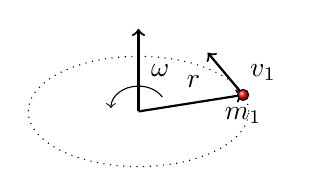
\begin{tikzpicture}[scale=.7]
  \draw[dotted] (1,.5) ellipse (2 and 1);
  \draw [<-,yscale=0.8] (.5,.7) arc (180:30:.5);

  \draw[->,thick] (1,.5)--(1,2); 
  \draw	(1,1.25)node[right=1pt]{$\vv{\omega}$};
     
\draw[->,thick] (1,.5) -- (2.9,.8);
\draw[<-,thick] (2.9,.8) +(130:1)--(2.9,.8)  ;
\draw (2,.7)node[above=1pt]{$\vv{r}$};
\draw	(2.8,1.2)node[right=1pt]{$\vv{v_1}$};
\draw (2.9,.8)node[below=1pt]{$m_1$};
\draw[shade,shading=ball,ball color=red] (2.9,.8) circle (.1);
 
\end{tikzpicture}
\end{boxleft}\begin{boxrightshaded}
\begin{align*}
\vv{a_t}	&=\vv{\alpha} \times \vv{r}\\
a_t		&=\alpha\cdot r \qquad \alpha \perp r \\
\vv{\alpha}	&=\vv{r} \times \vv{a_t}\\
\vv{v}		&=\vv{\omega}\times\vv{r}\\
v		&=\omega\cdot r  \qquad \omega \perp r\\
\vv{\omega}	&=\vv{r} \times \vv{v}\\
s		&=\varphi\cdot r  
\end{align*}
\end{boxrightshaded}

\begin{boxleft}\bla{Kreisfrequenz}
\des[\second]{T}{Periodendauer}\\
\des[\per\second]{n}{Drehzahl}\\
\des[\hertz]{f}{Frequenz}
\end{boxleft}\begin{boxrightshaded}
\begin{align*}
\omega&=\frac{2\cdot\pi}{T}\\
&=2\cdot\pi\cdot n \\
&=2\cdot\pi\cdot f
\end{align*}
\end{boxrightshaded}

\begin{boxleft}\bla{Radialbeschleunigung}
\des[\meter\per\second\tothe{2}]{a_r}{Radialbeschleunigung}
\end{boxleft}\begin{boxrightshaded}
\begin{align*}
a_r&=\frac{v^2}{r}\\
&=v\cdot\omega\\
&=\omega^2\cdot r
\end{align*}
\end{boxrightshaded}

\begin{boxleft}\bla{Umdrehungen}
\des{N}{Umdrehungen}
\end{boxleft}\begin{boxrightshaded}
\begin{align*}
N	&=\frac{\omega_0\cdot t}{2\cdot \pi}+\frac{1}{2}\cdot\frac{\alpha}{2\cdot \pi}\cdot t^2\\
	&=n_0\cdot t+\frac{\alpha}{4\cdot\pi}\cdot t^2
\end{align*}
\end{boxrightshaded}
